% !TeX document-id = {6d544fe2-4255-4108-8022-d809ff1d2c53}
% TeX program = xelatexmk %doesn't work, no xelatexmk option under 'build'. Changed default engine to xelatex (options-->configure-->build-->default build-->xelatex)
% see http://info.semprag.org/basics for a full description of this template
%\documentclass[times,linguex]{glossa}
\documentclass[12 pt]{article}
\usepackage[letterpaper]{geometry}
\usepackage{times}
\geometry{top=1.5in, bottom=1.0in, left=1.0in, right=1.0in}

\usepackage[hidelinks]{hyperref}
%\renewcommand{\sectionautorefname}{\S}
\usepackage{xcolor}
\hypersetup{
	colorlinks,
	linkcolor={blue!50!black},
	citecolor={blue!50!black},
	urlcolor={blue!80!black}
}


\usepackage{graphicx} %for images
\graphicspath{{images/}}
\usepackage{caption}
\captionsetup[table]{skip=0pt,singlelinecheck=off}
\captionsetup[figure]{skip=0pt,singlelinecheck=off}

\usepackage{booktabs}
\usepackage{enumitem} %customize list numberings

\usepackage[natbibapa]{apacite}
\usepackage{natbib}

\usepackage{tipa}
\newcommand{\nt}[1]{\textipa{[#1]}} % narrow transcription
\newcommand{\wt}[1]{\textipa{/#1/}} % wide transcription


\usepackage{fancyhdr}
\pagestyle{fancy}
\fancyhf{}
\renewcommand{\headrulewidth}{0pt}
\fancyhead[R]{\thepage}

\usepackage{setspace}
\doublespacing

\usepackage{comment}

\newlength\mystoreparindent
\newenvironment{myparindent}[1]{%
	\setlength{\mystoreparindent}{\the\parindent}
	\setlength{\parindent}{#1}
}{%
	\setlength{\parindent}{\mystoreparindent}
}

\usepackage{easyReview}

\title{Mixed language processing increases cross-language phonetic transfer in Bengali-English bilinguals}



% \author[Auromita \& Indranil]% short form of the author names for the running header. If no short author is given, no authors print in the headers.
% {%as many authors as you like, each separated by \AND.
%   \spauthor{Auromita Mitra\\ 
%   \institute{The EFL University}\\
%   \small{%105, Bd. Raspail, 75005 Paris\\
%   auromita.mitra@gmail.com}
%   }
%   \AND
%   \spauthor{Indranil Dutta \\
%   \institute{Jadavpur University}\\
%   \small{%Warmoesberg 26, 1000 Brussel\\
%   indranildutta.lnl@jadavpuruniversity.in}
%   }%
% }
%\usepackage{gb4e}

\begin{document}
\bibliographystyle{apacite}
%\sffamily
%\maketitle

%Word count: 9263

\begin{singlespace}

\begin{myparindent}{0pt}
Short title: Phonetic transfer\\

Full title: Mixed language processing increases cross-language phonetic transfer in Bengali-English bilinguals\\

Authors:\\

Auromita Mitra

EFL University,

Hyderabad,

India\\

Indranil Dutta

Jadavpur University,

Kolkata,

India\\

Acknowledgments:\\
We are grateful to Maumita Bhowmik and Anannya Mondal for their help with data collection and processing, and to all the participants of the study.\\
 

Address for correspondence:\\
Auromita Mitra,

EFL University,

Hyderabad- 500007,

auromita.mitra@gmail.com

\end{myparindent}

\end{singlespace}

\newpage
\begin{myparindent}{0pt}
Abstract:\\
This study investigates the phonetic outcome of mixed-language speech in Bengali and Indian English, towards understanding cross-language interaction in highly proficient bilinguals.  We compare spectral properties of L2 vowels \nt{\ae} (common to L1, L2) and \nt{2} (absent in L1) in unilingual vs. mixed productions. Results reveal dynamic and asymmetrical changes in both vowels;  \nt{2} shifting towards a related L1 category \nt{a:}. We interpret this as a temporary increase in cross-language phonetic interaction during mixed-language use, leading to a shift towards L1 norms, evidencing transfer effects on L2 vowels for the first time. We elicit mixed productions through two tasks: cued picture-naming and code-switching, to assess if experimental paradigm independently influences the behavior under study. Results reveal no difference across paradigms. We discuss these findings in light of recent proposals about asymmetries in short-term phonetic interaction, postulated discursive factors in code-switching, and the issue of comparability between paradigms in transfer studies.\\


Keywords: phonetic transfer; vowel quality; bilingual speech production; L1-L2 interaction; Indian English; Bengali 

\end{myparindent}

\newpage

\section{Introduction: Phonetic transfer}

Bi/multilingual speakers can distinguish between the phonetic norms of their languages and maintain separate sound categories for each language \citep{caramazza1973acquisition,macleod2010impact,bosch2003simultaneous}. However, these categories are not autonomous-- they influence each other across languages in both perception and production \citep[e.g.][]{flege1995second,fowler2008cross,flege2002assessing}, and the nature of such interaction provides crucial insights into how language `systems' are cognitively represented and processed. Based on the productions of proficient bilingual speakers of Bengali and English, this study reports that cross-language phonetic influence temporarily increases during mixed-language use.%Given that a majority of the world's population is multilingual, this is a central concern for any realistic theory of language.
%show cross-language-- rephrase

%keep just the types here, and put the next 2 lines in the causes&effects section?
Cross-language influence at the level of sounds can be studied in broadly two kinds of conditions:
(i) While a bilingual speaker is operating in any one of their languages, by comparing bilingual speech to monolingual norms \citep[e.g.][]{guion2003vowel,caramazza1973acquisition,flege1987production}; %These studies often compare the speech of bilinguals to monolingual norms, and view the influence as changes to long-term memory representations as a result of acquiring an L2 \citep{guion2003vowel,caramazza1973acquisition,flege1987production}; 
(ii) When both languages of a bilingual speaker are co-activated, by comparing speakers' mixed-language speech to their own norms while using a single language \citep[e.g.][]{grosjean1994going, bullock2009trying,elias2017effects, simonet2014phonetic}. %These compare productions during mixed-language use to participants' own productions while using a single language. The resulting influence is variously thought to involve short-term memory, online processing costs, language mode, and context-awareness. 
The present study is concerned with the latter. In production, this kind of influence has been variously termed \textsc{transfer, drift, accommodation,} and \textsc{interference}-- we use the term \textsc{transfer} here, to indicate any interaction between two sets of phonetic norms.

Existing research on the phonetic effects of mixed-language production has largely focused on a limited set of phonologically related languages. A majority of these studies use temporal properties of consonants (in particular, voice onset time or VOT) to measure transfer. However, the reported results vary greatly across studies, and appear to be contingent upon both language-specific features and language experience of the participants. This emphasizes the importance of considering data from a wider variety of
%elaborate on 'great variation'-- differences between language pairs, plus sociolinguistic situation (effects of language experience etc)-- clearer. 'Types of features'--separate line?- Brief mention - discursive factors in VOT. 
populations, language pairs,  and phonetic features in order to make meaningful generalizations. Widespread multilingualism in the Indian subcontinent suggests that phonetic
%line--rephrase
behavior in these populations can be particularly valuable towards understanding the nature of such cross-language interactions, as they are likely to reflect real-world experience with mixed-language processing. However, there is no work yet on short-term phonetic transfer in the Indian subcontinent, or in any Indo-Aryan language. 

The present study examines phonetic transfer between Bengali and English in a group of highly proficient bilingual speakers in India. We measure spectral properties: F1 and F2, of two English vowels to ascertain if L1 influence on L2 increases during mixed-language use, relative to a participant's unilingual baseline production of L2. Mixed-language data is elicited in two switching paradigms: cued picture-naming and code-switching. We compare these results to assess if differences between the paradigms independently influence the outcome of phonetic interaction. The results demonstrate a dynamic effect of transfer on L2 vowels during mixed-language production, \alert{but no difference in the extent of transfer between the two paradigms --and slightly different patterns of shift among the paradigms?}. We discuss these findings in light of recent proposals about asymmetries in short-term phonetic interaction and the role of connected speech in introducing discursive factors to transfer studies.


The rest of this section is structured as follows: \ref{bengali_english_in_india} provides background information on Bengali and Indian English focusing on vowel systems. \ref{causes} discusses two potential sources of transfer during language processing-- global co-activation of multiple languages vs. the local act of switching between languages. Given the highly multilingual setting that characterizes this population, we note that the former is expected to be a constant feature and therefore any observed phonetic interaction is better understood as resulting from the latter. The design of the present study is motivated on the basis of this discussion. A logical consequence of this model is that such phonetic interaction must be highly localized. \ref{duration} elaborates on this by reviewing literature on the duration and `reversibility' of transfer effects. A recurring pattern that emerges from existing research on short-term phonetic transfer is that both languages of the bilingual speaker are not equally affected, although the nature of these reported differences varies greatly across studies. In \ref{asymmetries}, we review some of these findings, focusing on proposed sources of asymmetries, in order to highlight the factors that mediate such phonetic interaction (or fail to do so). We argue that these results point to an urgent need for expanding the range of language pairs and sound categories examined in order to make meaningful generalizations about the nature of short-term phonetic transfer. Following from this, \ref{asymmetry between sounds} discusses reported asymmetries between different sound categories of a single language, and develops the hypotheses of the present study on the basis of these. In \ref{paradigms}, we motivate a secondary aim of this study: to verify the postulated differences between two paradigms for eliciting short-term phonetic interaction in an experimental setup, namely cued picture-naming and code-switching. \ref{questions_and_hypotheses} summarizes the research questions and hypotheses.

Existing studies have studied phonetic transfer along different acoustic features. While discussing the literature in subsequent sections, we will often indicate the acoustic feature in parentheses following a citation, for clarity. 

\subsection{Bengali and English in India} \label{bengali_english_in_india}

\subsubsection*{Demography} 

Bengali (also, Bangla) is an Indo-Aryan language primarily spoken in India and Bangladesh. In India, more than 97 million people speak Bengali as a first language (Census of India, 2011), mostly in the state of West Bengal. A majority of this population also speaks other additional languages.

Indian English (IE) refers to the variety of English that has developed in the Indian subcontinent. In India, it is spoken as an L2 by 129 million people (Census of India, 2011).  English is one of the two official languages, used in education, law, media, as a lingua franca mainly for an educated elite in most metropolitan regions, and carries a high prestige value \citep{pandey201517, kachru1981english, tollefson2014language, kachru1983indianization}.

\alert{note that there are large regional variations in Indian English, and the literature on IEphonology is thus not "standardized" or uncontested. For the present study, we focus on a variety of IE spoken by an educated elite, used in news channels, taught in classrooms (citations)}

Recent research comparing the segmental and suprasegmental properties of IE spoken in different parts of the country report many commonalities (see \cite{sirsa2013effects} for a review). This suggests that in spite of the varied L1s of its speakers, IE has a target phonology that is distinct from any of these, as well as from other native varieties of English. Thus, it is fruitful to think of regional variations as resulting from L1-influence on a common underlying target. Excepting a small minority of specific communities \citep{pandey201517, wells1982accents, coelho1997anglo}, there are very few L1 speakers of IE.


Considering the language usage patterns suggested by this demography, the present study focuses specifically on short-term phonetic interaction during mixed-language use, because:

\begin{enumerate}[label=(\roman*)]
	\item In multilingual populations, long-term representations of sound categories are expected to be affected by multiple languages. 
	\item Given that examples of an IE phonology without L1 `influence' are very rare, it is more meaningful to think of cross-language transfer in L2 as relative to a speaker's own production in a given baseline condition.
\end{enumerate}

The socio-linguistic facts about English in India also suggest that for the present population, mixed-language processing of English and an L1 is an ecologically valid paradigm that is likely to be a part of everyday language experience. Thus, data from this population is valuable to the understanding of short-term phonetic interaction.

\subsubsection*{Vowel systems} \label{vowel systems}
The vowel inventory of Western Bangla (the variety spoken by the participants in this study) consists of \nt{i, e, \ae, a, O, o, u}, and their nasalized counterparts \citep{garry2001facts}. Note that there is no mid-central vowel category. 


The vowel system of IE contains the monophthongs \nt{I, i, E, e, \ae, @/2, a:, O, o, U, u}, represented by the lexical set KIT, FLEECE, DRESS, FACE, and TRAP, STRUT, PALM, LOT/CLOTH, GOAT, FOOT, GOOSE \citep{wells1982accents, masica1972sound}. %Their distribution in the F1XF2 space is shown in (insert table 1.7, Pandey). 
A single mid-central vowel corresponds to the categories \nt{2,@,3:}, which are treated as distinct in many native varieties of English \citep{nihalani1979indian,wells1982accents,hickey2005legacies,bansal1969intelligibility}. Since the English items used in this study are traditionally transcribed with \nt{2}, we use this symbol to indicate the mid-central vowel throughout. 
 

\subsection{What causes transfer and what does it affect?}\label{causes}

Existing research has distinguished changes in category \textsc{representations} due to the acquisition of multiple sound systems (cf. Speech Learning Model \citep{flege1995second,flege2007language}; Perceptual Assimilation Model-L2 \citep{best2007nonnative}), from interaction during accessing, processing, or articulation of these categories (cf. transfer vs. interference \citep{grosjean2012attempt}; competence vs. performance interference \citep{paradis1993linguistic}). 
Given their transient nature, dynamic changes in production during mixed-language use are generally attributed to the latter, e.g. online processing costs \citep[][VOT]{olson2013bilingual,tsui2019impact,vsimavckova2015immediate}, language mode \citep[][vowel quality]{simonet2014phonetic}, context-awareness \citep[][phonological variables]{khattab2013phonetic}. What triggers this interaction? \cite{olson2016role} argues that while cross-language phonetic effects are largely measured at the point of language switch, it could have two potential sources:
\begin{enumerate}
	\item The local point of switch itself
	\item Global co-activation of two languages -- \textsc{bilingual language mode} \citep{grosjean1998studying} 
\end{enumerate}

A number of studies have specifically manipulated language mode, both in the presence and absence of switching. Overall, results suggest that: (i) In the absence of other manipulations, productions in a bilingual language mode show increased cross-language influence compared to a monolingual mode \citep[][vowel quality]{simonet2020increased,simonet2014phonetic}; (ii) However, language mode is not the sole source of influence during mixed language use--- studies comparing switched and non-switched tokens produced in the same test block (identical language mode) \citep[][VOT]{olson2016role,tsui2019impact} or spontaneous conversation \citep[][VOT]{piccinini2015voice}, have still reported a difference, suggesting that independently of mode, switching between languages triggers a local increase in cross-language transfer. (iii) How the two sources interact to influence the final outcome of transfer is not fully understood-- \cite[][VOT]{olson2016role} found no additive effects of language mode, \cite[][VOT]{olson2013bilingual} found a balanced language context to inhibit transfer compared to unbalanced contexts.  Other studies have not analyzed the two separately, eliciting switched tokens in a bilingual test block and non-switched tokens in a separate monolingual test block, separated by a few hours to days (\cite{elias2017effects}; vowel quality), \citep[][VOT]{schwartz2015language, bullock2009trying,antoniou2011inter, vsimavckova2015immediate,vsimavckova2018patterns}.

\cite{grosjean1998studying} suggests that various aspects of the communicative setting, including exposure to (spoken or written) stimuli in multiple languages and awareness of the interlocutor's being bilingual, could trigger a bilingual language mode. The participants in the present study are in an environment which largely contains mixed-language input, multilingual interlocutors, and no stable ambient language. Therefore we expect that phonetic transfer during everyday language use, if any, takes place in a bilingual mode.  To preserve ecological validity, we elicited both unilingual and switched utterances in a bilingual language mode. Any observed differences in this paradigm would arguably result from interaction during online processing of sounds while switching between languages. 

In a bilingual mode, both language systems are expected to be nearly equally accessible throughout the test block. Thus, a consistent difference between switched and non-switched tokens in such a paradigm would be possible only if the effects were highly localized-- if not, we should expect a gradual convergence over the course of the experiment. This is discussed in the next section.


\subsection{Duration of transfer effects} \label{duration}

Research comparing bilingual speakers' phonological systems with monolinguals treats them as relatively stable over time. The difference from monolingual norms is interpreted as the cumulative result of cross-language influence over long periods \citep[e.g.][]{guion2003vowel, caramazza1973acquisition}. However, longitudinal studies %(citations) 
and between-subject comparisons of bilingual speakers with different durations of L2 exposure suggest that interaction between the sound systems is dynamic: over time, increasing exposure to an L2 can reduce effects of L1 influence, leading to a more fine-grained separation and native-like production of foreign contrasts. For example, \cite[][vowel quality]{bohn1992production} 
observed that approximately 7 years' difference in L2 exposure between groups having the same age of acquisition led to a significant difference in the amount of cross-language influence. These have been interpreted as changes to long-term phonological representations.

Moreover, changes due to transfer are not necessarily unidirectional or irreversible. \cite[][VOT]{sancier1997gestural} first demonstrated that spending 2-5 months in an L1 or L2 environment causes productions in both languages to ``drift" towards the ambient language. This not only evidenced that cross-language interaction can be triggered in an order of months, but also that the effects can be reversed within a similar time range. A more recent study by \cite[][VOT]{tobin2017phonetic} reported comparable effects in an even shorter duration (2-4 weeks). Based on a short-term longitudinal study, \cite[][VOT]{chang2012rapid} demonstrates that over the course of the first five weeks of learning an L2, there is a gradual convergence of L1 towards L2. For some sounds and features (though not others, cf. sec.\ref{asymmetry between sounds}), transfer was additive over time. How long these effects last in the absence of regular L2 input was not tested. 
% if effects are cumulative, then the difference between switched and non-switched tokes should be lesser in later test blocks (previous two paragraphs needed?)

The research discussed above concerns situations where a speaker is operating in any one of their languages. When it comes to the phonetics of mixed-language use, the majority of existing studies only analyze the switched (target) token. Thus, there are few direct measurements of the duration of short-term transfer effects. One study which measured this in a code-switching paradigm \citep[][VOT]{bullock2009trying} did not find any residual effects on the matrix language following a switch, suggesting that transfer during code-switching is localized. Indirect evidence in support of this comes from experiments which have elicited switched and non-switched tokens in the same test block and still reported differences between the two \citep[e.g.][VOT]{tsui2019impact,olson2013bilingual}, suggesting that changes due to transfer are quickly `reset'--- in an order of seconds.\\
Note that all the studies discussed above measure VOT, which is a temporal feature. We have no apriori reason to assume that these durations generalize to vowel quality. However, findings from sub-categorical phonetic shifts triggered by other factors (such as convergence towards an interlocutor) do evidence rapid shifts in vowel quality within comparable time-frames \citep[e.g.][]{pardo2010expressing,babel2010dialect,babel2012evidence}. Thus in the current study, we present switched and non-switched tokens randomly within the same test block to induce a bilingual mode. We expect the intervening words between two subsequent targets to undo any residual effects of transfer.

\alert{discussion: found that like VOT, vowel quality shifts due to switching are also highly localized, and reset in an order of seconds. This behavior is similar to other context-driven shifts in the literature}

\subsection{Asymmetries between languages in extent and direction of transfer} \label{asymmetries}
A recurring pattern that emerges from existing research on short-term phonetic transfer is that the extent and patterns of phonetic shift are not equivalent across the two languages of the bilingual speaker. Studies vary greatly in the nature of differences that they report. The potential causes for such asymmetry are of interest because they point towards the factors that mediate cross-language phonetic interaction. In this section, we discuss two proposed sources of such asymmetry that are relevant to the present study: 

\subsubsection*{L1 vs. L2 status} 
Flege's Speech Learning Model (SLM) \citeyearpar{flege1995second,flege2007language} posits that the sound categories of a bilingual speaker exist in a common phonological space, and therefore in principle, both L1 and L2 categories can influence one another. Thus, the patterns of cross-language transfer depend on how L2 phonemes are mapped in relation to the existing L1 categories. In non-switched production, this is evidenced through a pervasive L1 influence on non-native contrasts that are perceptually linked to an existing L1 contrast (cf. \textsc{equivalence classification}-- \cite{flege1984limits,flege1987production}), and the observation that both L1 and L2 sound systems of bilinguals differ from those of corresponding monolingual speakers \citep[e.g.][vowel quality]{guion2003vowel}. 

In mixed-language production, the role of language status is less clear-- studies have reported unidirectional influence of L1 on L2 \citep[][VOT]{balukas2015spanish,antoniou2011inter,vsimavckova2015immediate,goldrick2014language}, L2 on L1 \citep[][VOT]{tsui2019impact, olson2013bilingual}, (\cite{elias2017effects}, vowel quality) bidirectional convergence \citep[][VOT]{bullock2009trying, olson2016role}, divergence \citep[][VOT]{bullock2009trying,vsimavckova2018patterns}, and no influence \citep[][vowel quality]{muldner2019phonetics}, \citep[][phonological process]{schwartz2015language}. Since most existing studies measure shifts in VOT, the observed asymmetries between languages have been variously explained either in terms of their L1 vs L2 status, or language-specific differences between long- and short-lag VOT languages. %(cf sec. \ref{sound systems}).

\cite{olson2013bilingual} first reported a unidirectional VOT shift of L1 towards L2 in two different groups -- native speakers of Spanish (short-lag) and English (long-lag), matched for proficiency and age of L2 acquisition. This established that beyond language-specific differences, the L1 vs L2 status of the language does mediate transfer. They interpret this asymmetry in terms of the Inhibitory Control Model (ICM) \citep{green1998mental}: to select a phonetic realization from one language, the other must be \textsc{inhibited}. Since L1 is the `stronger' language, the amount of inhibition required on L1 while using an L2 is greater than the inhibition required on an L2 while using the L1. This greater initial inhibition on L1 means that switching into L1 incurs a greater \textsc{switch cost} (more cross-language influence) than switching into L2. Lower switch cost results in a lack of visible cross-language transfer effects on L2. \cite{tsui2019impact} report comparable results, but only in participants who were not equally dominant in both languages. Balanced bilinguals did not demonstrate any transfer effects in VOT. They propose that this is because balanced bilinguals have better inhibitory control (low switch cost in both languages) due to greater experience with language switching.

Since differences between long-lag and short-lag languages independently affect the phonetic realization of VOT, focusing on other phonetic features as sites for transfer can avoid this conflation, and clarify the precise effect of language status. However, given the implications of the ICM, it is necessary to first establish that these L2 categories can indeed be affected by dynamic interference, particularly in bilinguals with extensive language-switching experience. The few existing studies on vowel quality \citep{simonet2014phonetic,muldner2019phonetics,elias2017effects} or phonological processes \citep{simonet2020increased,schwartz2015language} have examined transfer effects on L1 categories. As far as we are aware, there is no work yet on short-term transfer in L2 vowels. Thus, this study builds on the existing work by examining whether the L2 vowel quality of proficient bilinguals can be affected by mixed-language processing.

\alert{discussion: more about ICM, assumptions about processing}

\subsubsection*{Differences between sound systems of the languages} \label{sound systems} In addition to the cognitive factors discussed above, many researchers have attributed the observed asymmetries to language-internal factors. Specifically, a pattern that emerges from the body of work on VOT is that a shift in long-lag VOT towards the short-lag norms of the other language is much more consistent and systematic than the converse \citep{tobin2017phonetic, olson2016role,bullock2009trying,antoniou2011inter,chang2012rapid}. In general, short-lag VOTs seem to resist accommodative shift. \cite{bullock2009trying} suggest that because long-lag languages offer a greater range of acceptable VOTs, there is more `room' for movement. In contrast, shift in short-lag languages could risk the loss of a phonological contrast (VOT being the primary cue for voicing contrast in these languages).  This is a language-specific phonological constraint on transfer.
In a similar vein, \cite{antoniou2011inter} observe that while the VOT of English stops shifted towards Greek (a short-lag language), the reverse was seen only in a specific subset of sounds-- word-medial non-nasalized stops. They attribute this to the low frequency of these sounds in Greek, making them less ``stable", and thus more amenable to cross-language influence. This suggests that the distribution of sounds in a language could affect the kind of transfer patterns observed.

These results highlight that beyond interaction during the cognitive processing of sounds, phonetic transfer is ultimately a linguistic phenomenon, and thus subject to language-specific phonological constraints. Therefore, to make meaningful generalizations, it is imperative to consider data from a variety of language pairs. Existing research on phonetic transfer largely revolves around a limited set of phonologically related languages. Thus, the present study extends the scope of this research to a new pair of languages--- Indian English and Bengali.

Since Bengali has a four-way laryngeal contrast, VOT does not encode a binary voiced-voiceless distinction. Moreover, VOT is not the only relevant cue for the corresponding phonological categories in the language \citep{dmitrieva2020acoustic}. This means that any effect of L1 Bengali on L2 English VOT is likely to be affected by additional phonological factors. Thus, avoiding any potential confounds was another reason we chose to focus on vowel quality as a target for transfer in the present study. 


\subsection{Asymmetries between sounds}\label{asymmetry between sounds}

Asymmetries in the extent and patterns of transfer have not only been observed between languages, but also between different sounds/features of a language, in both long-term and transient interactions. Studies that have examined multiple sound categories have found that interactions between individual sound pairs do not necessarily reflect the overall pattern of global (system-wide) shift \citep[e.g.][vowel quality]{chang2012rapid,elias2017effects}, suggesting that `extent of transfer' cannot treated as an atomic measure. In light of the discussion about VOT in section \ref{sound systems}, this is not surprising --- if a general linguistic principle of `room for movement' and contrast constrains transfer, then we should expect it to apply to individual sounds too. Once again, this emphasizes the importance of examining a wider range of sound contrasts.


In the present study, we focus on two vowel categories in Indian English-- the mid-central vowel \nt{2} and the low front vowel \nt{\ae}. There are two plausible sources of asymmetry between these:
\begin{enumerate}
	\item Position in the IE vowel space: compared to \nt{\ae}, \nt{2} exists in a part of the vowel space that has a lower vowel density. This affords a greater latitude for movement without risking the loss of a contrast, particularly in the vowel height (F1) dimension. Thus, considering purely phonological constraints on IE, we expect that a greater degree of shift is possible in \nt{2} compared to \nt{\ae}. Any movement in \nt{\ae} is expected to be primarily in the backness (F2) dimension.
	\item Target of transfer: findings from existing research on cross-language phonetic interaction suggest that changes in production during mixed-language use are not random, but rather targeted with respect to categories in the other language. Thus, another source of asymmetry is the fact that the category \nt{2} is absent in Bengali, whereas \nt{\ae} is a common category across both languages (cf. sec.\ref{vowel systems}).
\end{enumerate}

%table

Flege's Speech Learning Model (SLM) \citeyearpar{flege1995second,flege2007language} posits that sound categories which are common across languages influence each other because they share a common acoustic-phonetic space. Thus, if Bengali and English differ in their canonical realizations of \nt{\ae}, then we should expect the English \nt{\ae} to shift towards the corresponding Bengali category in the mixed condition. 

%Other categories can in principle be produced with native-like accuracy, showing little effect of transfer. Given that our participants are highly proficient bilinguals, and assuming that cross-language correspondences remain the same in representation and processing, this would lead us to expect more transfer in the common category, \nt{\ae}. 

There is no obvious competing L1 category during the production of \nt{2}. However, it is unlikely that this should altogether preclude a shift in \nt{2}, since at least one existing study has reported transfer effects on a non-common vowel category in a comparable paradigm \citep{simonet2014phonetic}. Here, participants' Catalan \nt{O} shifted towards an acoustically close category \nt{o}, which is common to Catalan and Spanish, suggesting that movement might be towards a set of phonetic norms rather than a specific corresponding category. 

We expect the vowel \nt{2} to shift towards an acoustically/perceptually close category in IE -- a probable candidate being the low vowel \nt{a:}, as anecdotal observations of Bengali-accented English suggest that the sounds are perceived as close by Bengali speakers. 


In the present study, our research question concerns whether L2 vowels are produced differently in unilingual vs mixed conditions. We do not elicit unilingual Bengali productions. To estimate average baseline differences in vowel quality between the relevant English and Bengali categories, we used production data from the freely available Bengali corpus, SHRUTI \citep{shruticorpus}. Formant values were extracted from syllable-initial productions of \nt{\ae} and \nt{a:}, at 55\% into the vowel, to get formant estimates from the steady state, which should most closely approximate the production target. Next, we compared these to our participants' productions in the unilingual English condition to understand the relative positions of the categories. \alert{fig. .. plots-- from current plot- remove the dotted line. Filter by context, then remove group=context from figure code} F1-F2 plots show that the Bengali category \nt{\ae} is lower, and \nt{a:} lower and more fronted, than the English categories \nt{\ae} and \nt{2} respectively. 

\subsection{A note on paradigms: connected speech or not?} \label{paradigms}

This section motivates a secondary aim of this study: to verify if the extent and patterns of phonetic interaction in bilingual participants are independently mediated by the choice of experimental paradigm. Studies of phonetic transfer during mixed-language use have largely employed spontaneous or scripted code-switching (CS) to elicit mixed productions. CS is defined as the use of multiple languages within a single utterance, i.e. in connected speech \citep{myers1993dueling}. Other paradigms which have been used include cued picture-naming, delayed repetition, interpreting across languages, reading word-lists etc. \cite{olson2013bilingual} argues that code-switching introduces discursive factors such as discourse planning and pragmatic considerations, which ultimately reflect patterns of language practice, rather than cognitive behavior. This finds support from studies which report transfer effects \textsc{before} the switch point \citep{bullock2009trying}, or other evidence for planning such as hyperarticulation \citep{muldner2019phonetics} and interlocutor-awareness in spontaneous CS \citep{khattab2013phonetic}. To avoid such confounds, \cite{olson2013bilingual} endorses cued picture-naming (where pictures are named in rapid succession in either language, based on the given language cue) as an alternative paradigm to isolate purely phonetic effects in controlled setups. This observation has important implications for how the existing literature on short-term phonetic interaction is interpreted: if the discursive properties of a CS paradigm independently affect the phonetic outcome of mixed-language use, this calls to question the comparability of results across studies using these different paradigms. Because the reported outcomes of short-term phonetic interaction vary so greatly across studies (cf. section \ref{asymmetries}), generalizations about the mechanisms that underlie these patterns often rely crucially on the assumption of such comparability. Therefore, identifying paradigm-specific differences is particularly relevant for this line of research.

Note that while there is evidence for planning in CS, precisely how this affects phonetic interaction cannot be predicted from the existing literature--- while \cite{bullock2009trying} found tokens immediately preceding the switch point to be phonetically distinct from the rest, one participant group converged towards the switch language (explained in terms of proficiency) while the other showed divergence (explained in terms of extra-linguistic factors). The participants in Muldner et al.'s \citeyearpar{muldner2019phonetics} study hyperarticulated switched tokens (indicating some degree of planning), and did not evidence a significant shift during mixed-language use. Moreover, recall that the findings of \cite{olson2016role} suggest that there is a limit on the extent of transfer--- multiple factors do not necessarily result in additive effects. Thus, the presence of additional factors in CS does not necessitate that this should alter the extent of observable transfer compared to any other paradigm. It is possible that the outcomes in the studies discussed above are better attributed to some other aspect of the experimental setup, rather than to the act of code-switching in particular.

The precise contribution of various (linguistic and extra-linguistic) factors and their interactions to the phonetics mixed-language use merits detailed investigation in its own right. In the present study, however, our focus is limited to verifying whether, in an experimental setting, the postulated discursive elements of a CS paradigm alter the extent of observable transfer compared to a paradigm that arguably lacks these--- cued picture-naming. We are less concerned with the exact nature of differences than with their comparability. While researchers have successfully employed each of these paradigms to induce phonetic interaction, comparison across studies is difficult since they also differ in other factors. We provide a starting point for such comparison by eliciting productions of the same tokens from the same set of participants, in both paradigms. A difference in results will suggest that the planning involved in connected speech and code-switching affects transfer above and beyond the phonetic outcome of switching itself, which has implications that future work should consider. 


\subsection{Research questions and hypotheses}\label{questions_and_hypotheses}
\begin{itemize}
	\item \textbf{L2 vowels}: Are L2 vowel categories of proficient bilingual speakers affected by dynamic phonetic transfer during mixed-language production, as evidenced by differences in the spectral properties of L2 vowels in switched and non-switched tokens?
	\item \textbf{Asymmetry}: If so, we expect an asymmetry between the vowels in the extent and direction of shift. Based on comparisons with Bengali vowels from \cite{dutta2021} we expect \nt{2} to be lowered and fronted in the mixed condition. \nt{\ae} is expected to show lowering, but to a lesser extent than \nt{2}, as it is in a part of the IE vowel space that has greater vowel density.
	\item \textbf{Paradigm}: Is there an observable difference between the extent of transfer in a cued picture-naming vs. a code-switching paradigm? 
\end{itemize}


\section{Methodology} \label{methodology}
The experiment had the following factorial design: 10 participants* 20 target words* 2 conditions* 2 tasks* 4 iterations = 3200 target tokens.

\subsection{Participants} \label{participants}

10 Bengali-English bilingual speakers (male=5, age range 19 to 28), completed the tasks. All the participants speak other languages in addition to Bengali and English. At the time of recording, they were living in or around the EFL University campus in Hyderabad, which has a linguistically diverse population. Speakers were selected on the basis of responses to a Language Background Questionnaire to ensure comparable LSRW (listening, speaking, reading, writing) skills in L1 and L2 across participants, and were compensated for their time.


\subsection{Stimuli}
Twenty monosyllabic English words containing the vowels \nt{2} or \nt{\ae} were selected as target words. To minimize coarticulatory effects on the vowel, the pre-vocalic consonants were all voiced plosives (\nt{b} or \nt{d}). 10 monosyllabic English words that do not contain the target vowel served as filler items. We avoided English words that are lexicalized loanwords in Bengali. %The list of words can be found in sec.\ref{appendix}.



\subsection{Procedure}
Participants were recorded individually in a sound attenuated room. %, using a ... microphone type/description?
Productions were recorded in Praat \citep{boersma2016praat} at a 44.1K sampling rate. Every participant performed four iterations each of two tasks-- cued picture-naming and code-switching. Utterances in the two conditions (unilingual and mixed) were randomly interspersed within each iteration. In the unilingual condition, the target word was preceded by another English word in the utterance. In the mixed condition, the target was preceded by a Bengali word and thus produced as a switch from Bengali. Every target word appeared twice during a test block; once in a unilingual and once in a mixed condition. Participants alternated between the two tasks, and were allowed to take a short break after each test block. The tasks are described below:


\begin{enumerate}[]
	\item Cued picture-naming: Participants were presented with slides in the following sequence:
	\begin{itemize}
		\item Language cue- a word in either English or Bengali orthography
		\item A picture displayed for 50ms; named by the participant in either English or Bengali, depending on the language cue 
		\item Target -- an English word; read out by the participant
		\item Distracter math problem
	\end{itemize}
	Since all the target words were in English, the language cue was used to manipulate the \textsc{preceding} word, giving target words in non-switched (unilingual) and switched (mixed) utterances. The orthographies of English and Bengali are visually distinct, and were therefore used to cue language.
	
	\item Code-switching: Each slide contained one target word embedded in either an English (unilingual) or a Bengali (mixed; target produced as a switch from Bengali) carrier sentence which was read out by the participant. The carrier sentences are given below:
	\begin{itemize}
		\item Unilingual sentence: That is a yellow [\textit{target word}].
		\item Mixed-language sentence: \textipa{o-\:ta \ae k-\:ta kalo} [\textit{target word}]. 
	\end{itemize}
	
Gloss and translation for Bengali sentence:

o-\textipa{\:t}a \qquad \textipa{\ae}k-\textipa{\:t}a \quad kalo [\textit{target word}]\\
that-\textsc{clf}  one-\textsc{clf}  black [\textit{target word}]\\
``that is a black [\textit{target word}]"\\
	
The sound preceding the target word was uniform across all sentences (the final sound in \textit{yellow} is produced as [o] in Indian English), to minimize any possible differences due to coarticulatory effects on the target vowel. A specifier-noun construction was used to ensure identical word order in both languages, giving a uniform prosodic context for the target word across condition. In presenting the mixed-language utterances, we used mixed orthography. \\
	
\end{enumerate}
\subsection{Acoustic analysis}\label{analysis}
The first iteration of each task was treated as a trial, and excluded from further analyses. An additional 67 tokens (2.79\%) were excluded due to errors in presentation/production, giving 2333 target word tokens (\nt{2}: 1137, \nt{\ae}: 1196) for analysis. Recordings were manually segmented and annotated in Praat \citep{boersma2016praat}, and the first and second formant frequencies (F1 and F2) of the target vowels \nt{2, \ae} were measured at five points-- in 10\% increments starting at 5\% into the vowel. This gave measures of F1 and F2 at 5\%, 15\%, 25\%, 35\% and 45\% into the vowel, allowing us to observe any dynamic changes in the extent of transfer over the course of producing the vowel. Individual vocal tract differences affect formant frequencies across speakers. To avoid this confound, we used Lobanov normalization (using the PhonR package \citep{phonR} in R \citep{r}, representing each speaker's formant frequencies as the scaled distance from their own mean (\alert{citation for lobanov normalization?}). Plotting the vowels \alert{(figure)} shows a difference between male and female speakers, such that male speakers have overall lower formant frequencies. Speaker normalization using the Lobanov method does not get rid of this difference. Since gender-related differences in formant frequencies are not of interest in this study, we normalized individual values by gender (representing each value as a scaled distance from the group mean). Statistical analyses were performed on these normalized values. 


\section{Results} \label{results}

All statistical analyses were performed in R \citep{r}. We used linear mixed effects models to test the effect of experimental conditions on vowel height (F1) and backness (F2) respectively. Since formants were extracted from five points over the course of articulating the vowel, time was coded numerically (1-5), and treated as an independent variable. This was scaled and centered prior to analysis and treated as a continuous predictor. We fitted models using the \emph{lme4} package \citep{lme4}, and used \emph{lmerTest} \citep{lmerTest} to obtain estimates of p values for individual variables. For all mixed models, the alpha criterion was set at $|t| > 2 $. The dependent variables were normalized F1 and F2, and we fitted separate models for these. The independent variables or fixed factors, along with their levels, are given in table \ref{table variables} \alert{add variable type with each: factor, numerical, ...}. Subject and Item were treated as random factors.\\

< Insert Table \ref{table variables} about here > \\

\subsection{Models}

\subsubsection*{Fixed effects}

Our study involved two IE vowels. Vowel category is expected to systematically affect formant frequencies (FFs). 

The experimental treatment of interest is Context, i.e. whether the target item was presented in a unilingual (English) or mixed (Bengali) context. Our main research question (\bf{L2 vowels}) asks whether L2 vowel quality (formant frequencies) of proficient bilinguals is affected by the Context of utterance. We hypothesize that the direction of shift in the mixed condition is towards the corresponding L1 category. Thus, we expect the effect of Context on formant frequencies, i.e. the direction of shift, to be affected by the vowel category (c.f. section \ref{asymmetry between sounds}). Thus, our main effect of interest is the interaction term Context*Vowel. This corresponds to the transfer pattern.

Our third research question (\bf{Paradigm}) asks whether the language-mixing paradigm, or Task, affects the extent and direction of transfer. If this is the case, we expect Task to interact with the transfer term, giving a three way Task*Context*Vowel interaction.

Since we measured FFs at five points in the vowel, Time is expected to affect the FF. However, the precise effect of formant dynamics is expected to depend on the vowel category. Thus, we expect the interaction of Vowel*Time to predict formant frequency. If transfer patterns change across time, then we should expect it to interact with the transfer term, giving a Context*Vowel*Time interaction.

\subsubsection*{Random effects structure}

Subject and Item were treated as random factors. Given our hypotheses, we included random intercepts for Subject and Item, by-subject random slopes for Vowel (formant targets for vowel categories differ across individuals) and Context (individuals differ in their response to the experimental condition), and a by-item random slope for Context (the effect of experimental conditions differ across words). 

We tested the significance of our hypothesized explanatory variables using t-values and p-values for individual variables in the models, and tested overall model fit by comparing the full model to a corresponding null model that lacks the variable of interest using ANOVAs. The following subsections summarize and discuss the model outputs for F1 and F2 respectively.



\subsection{Vowel Height -- F1}

\subsubsection*{Model output summary}

First, to test hypothesis 1 (\bf{L2 transfer}), we fitted a model with vowel*time, and vowel*context as fixed effects. The transfer term (vowel*context) is significant in this model (model coefficient/ unstandardized effect size ($\beta$)= -2.330e-01, standard error (SE)=  5.244e-02, t= -4.44, p=0.0002). Comparing this to a null model that lacks the transfer term shows that the full model is significantly better ($\chi^2(2) = 14.42, p=  0.0007$). To confirm whether the effect of context is moderated by vowel identity, we compared a second null model that contained Context as a fixed effect, but lacked the Context*Vowel interaction. The full model was better ($\chi^2(1) = 12.51, p= 0.0004$).

To test the hypothesis \textbf{Paradigm}, we fitted a model with vowel*time and task*vowel*context as fixed effects. This three-way interaction term is significant ($\beta$= -1.955e-01, SE=  5.453e-02, t= -3.59, p= 0.0003). We also find a significant effect of task on FFs ($\beta$=3.300e-01, SE=2.668e-02, t=12.371, p=2e-16). Comparing this model to null models that lack the fixed effect Task ($\chi^2(4) = 572.61, p=  2.2e-16$) shows that the full model is better. Because Task has an independent effect on F1, and adding interactions increases model parameters, we fitted a second null model with Task as a separate fixed effect without the interaction term to test whether the interaction term is needed. However, the full model was still a better fit for the data ($\chi^2(3) = 23.82, p=  2.722e-05$). Next, we tested two other null models to verify that the full model with the three-way interaction term is indeed the optimal model for the data, by replacing the three-way interaction term with: (i) vowel*context + task*context (to test if task only interacts with context, rather than the transfer term vowel*context). The full model is better ($\chi^2(2) = 23.28, p= 8.78e-06$); (ii) vowel*context + task*vowel (to test if task only interacts with vowel, rather than the transfer term vowel*context). The full model is better ($\chi^2(2) = 13.36, p= 0.001$). This shows that the three-way interaction is the best fit for the data. Because an independent effect of task on FFs is unexpected (c.f. ), we wanted to see if the effect might be local, i.e. decrease over time. We added a task*time interaction term to the full model, which is significant ($\beta$= -1.216e-01, SE=  1.347e-02, t= -9.028, p= 2e-16 ) and improves model fit ($\chi^2(1) = 81.22, p= 2.2e-16$).

Next, to examine the dynamics of transfer, we added a three-way interaction between the transfer term (vowel*context) and time. This term has a marginally significant effect ($\beta$= -4.604e-02, SE=  2.692e-02, t= -1.71, p= 0.08), but does not significantly improve model fit compared to a null model lacking the vowel*context*time term ($\chi^2(2) = 3.41, p= 0.18$).

Thus, the optimal model was: f1 ~ time*vowel + vowel*context*task + time*task + (1 + context|word) + (1 + context + vowel|subject). Table \ref{table_f1} summarizes the model coefficient estimates ($\beta$), standard errors (S.E.), t-values, and p-values for this model. \alert{p-vales smaller than 0.05 are in bold.} 


\subsubsection*{Interpretation}
We extracted formant estimates from five uniformly spaced points in the vowel, from the time at 5\% into the vowel (at the start of articulation) to 45\% (at the mid-part, or steady state, which is expected to correspond to the articulatory target for the category). As expected, we see that F1 values are significantly predicted by Time in the model, reflecting th dynamic nature of articulation which causes acoustic variation over the course of time. The positive slope of the estimate for Time indicates that F1 increases, i.e. the two categories in the study show lowering over the course of articulation. Moreover, the significant Time*Vowel interaction shows that the F1 trajectory is different for the two vowels. This is expected, as the categories are expected to present different articulatory targets.  

 Vowel is not a significant predictor of F1. This appears surprising, given that the phonological category is expected to systematically affect vowel quality. However, a boxplot visualization (Figure \ref{boxplot_F1}) shows that the participants in this study vary greatly both in the relative heights of the two categories \nt{2, \ae} and the extent of height difference between them. Note that these measures are only from the English (unilingual) condition, suggesting that this variability is a feature of the participants' IE vowel categories, independent of the effects of switching. Given that estimates for fixed effects are pooled across participants, this explains the lack of reliable differences between \nt{2} and \nt{\ae}. The negative slope of the estimate for Context shows that F1 is lower, i.e. vowels are higher, in the unilingual (e) condition compared to the mixed (b) condition. Put more intuitively, vowels are lowered in the mixed condition. However, the lack significance indicates that using English words in mixed utterances does not lead to a uniform lowering/raising across vowels. Instead, the significant interaction between Vowel and Context signals an asymmetrical shift in the categories \nt{2} and \nt{\ae} in the mixed-language condition. Specifically, the Vowel*Context interaction has a negative slope, showing that the lowering is greater in \nt{2}.  
 
The results also reveal a significant effect of Task, such that the sentence task (code-switching) leads to higher F1 values in both vowels relative to the cued picture-naming task as: vowels are lowered in the code-switching task, independent of experimental condition. This is surprising, as we have no aproiri reason to expect a uniform difference in vowel quality across tasks. A significant interaction with Time with a positive slope of the estimate shows that this effect is local: it is strongest at the beginning of the vowel, and reduces over the course of the vowel. This is consistent with our assumption that the unexpected Task effect is an artifact of the paradigm, possibly resulting from coarticulatory effects with the preceding sound in the carrier phrase. Of greater interest to us is the significant Vowel*Context*Task interaction, which indicates a difference in transfer patterns across paradigms. Specifically, the negative slope of the estimate suggests that transfer in the F1 (height) dimension are greater in the code-switching (s) task compared to the picture-naming (p) task.\\


< Insert Figure \ref{boxplot_F1} about here >\\


\subsection{Vowel backness -- F2}

\subsubsection*{Model output summary}

First, to test hypothesis 1 (\bf{L2 transfer}), we fitted a model with vowel*time, and vowel*context as fixed effects. The transfer term (vowel*context) is significant in this model (standardized effect size ($\beta$)= 1.234e-01, standardized error (SE)=  2.055e-02, t= 6.00, p=5.46e-06). Comparing this to a null model that lacks the transfer term shows that the full model is significantly better ($\chi^2(2) = 16.20, p= 0.0003$). To confirm whether the effect of context is moderated by vowel identity, we compared a second null model that contained Context as a fixed effect, but lacked the Context*Vowel interaction. The full model was better ($\chi^2(1) = 16.02, p= 6.245e-05$).
  
To test the hypothesis \textbf{Paradigm}, we fitted a model with vowel*time and task*vowel*context as fixed effects. While task has an independent effect on F2 ($\beta$= -8.758e-02, SE= 1.756e-02, t= -4.98, p= 6.18e-07), the three-way interaction term is not significant ($\beta$= 3.349e-02, SE= 3.565e-02, t= 0.94, p= 0.34). However, there are significant two-way interactions between task*context ($\beta$= -1.099e-01, SE= 2.483e-02, t= -4.427, p= 9.66e-06) and task*vowel ($\beta$= -8.983e-02, SE= 2.535e-02, t= -3.544, p= 0.000396). Comparing this to a null model that lacks the fixed effect Task confirms that the full model is still a better fit for the data ($\chi^2(4) = 572.61, p=  2.2e-16$), indicating that an optimal model should contain the term Task. To confirm whether Task interacts with any of the other terms, we fitted a model with Task as a separate fixed effect without the interaction term. Comparing this to the full (interaction) model shows that the latter is still a better fit ($\chi^2(3) = 44.8, p= 1.02e-09$). Next, we tested two other null models to verify that the three-way interaction term is indeed optimal for the data, by replacing the three-way interaction term with: (i) vowel*context + task*context (to test if task only interacts with context, rather than the transfer term vowel*context). The full model is better ($\chi^2(2) = 17.28, p= 0.0001$); (ii) vowel*context + task*vowel (to test if task only interacts with vowel, rather than the transfer term vowel*context). The full model is better ($\chi^2(2) = 28.45, p= 6.633e-07$). This shows that the three-way interaction is the best fit for the data.

Because an independent effect of task on FFs is unexpected \alert{(c.f. next section)}, we wanted to see if the effect might be local, i.e. decrease over time. We added a task*time interaction term to the full model, which is significant ($\beta$= 6.237e-02, SE=  8.876e-03, t= 7.027, p= 2.23e-12 ) and improves model fit ($\chi^2(1) = 49.271, p= 2.23e-12$).
	
Next, to examine the dynamics of transfer, we added a three-way interaction between the transfer term (vowel*context) and time. This term is not significant ($\beta$= -6.274e-03, SE= 1.774e-02, t= -0.35, p= 0.72), and the addition does not significantly improve model fit compared to a null model lacking the vowel*context*time term ($\chi^2(2) = 2.2443, p= 0.32$).

Thus, the optimal model is: vowel*time + vowel*context*task + task*time + (1+context|word) + (1+context+vowel|subject). Table \ref{table_f2} summarizes the model coefficient estimates ($\beta$), standard errors (S.E.), t-values, and p-values for this model. \alert{p-vales smaller than 0.05 are in bold.} 


Statistical analyses reveal that the vowel \nt{2} is lowered and fronted, while \nt{\ae} is fronted, in the mixed condition.  Previous literature on phonetic transfer suggests that such shifts are not random, but rather directional and targeted. We want to understand how the direction of shift compares to corresponding Bengali categories. Figure \ref{vowels_e_b} summarizes the findings of the experiment ($F1XF2$ plots for vowel productions in the unilingual and mixed conditions, in comparison to the related Bengali categories from \cite{dutta2021}). This confirms our hypotheses (c.f. section \ref{asymmetry between sounds}) that \nt{\ae} moves towards the corresponding \nt{\ae} category in Bengali, whereas the shift in \nt{2} is towards the related Bengali category \nt{a:}. The following sections discuss the results for vowel height and backness respectively.

< Insert Figure \ref{vowels_e_b} about here >

\subsection*{Interpretation}

As with F1, we find that Time significantly influences F2 values in the model, reflecting the dynamic nature of articulation which causes acoustic variation over the course of time. Moreover, the Time*Vowel interaction shows that this trajectory differs across the two vowels: while the positive slope for Time indicates that F2 increases, i.e. vowels are fronted with time, the negative slope of the Time*Vowel interaction shows that this effect is smaller for \nt{2}. This is expected, as figure \alert{ref} confirms that the category \nt{\ae} is overall more fronted than \nt{2}. 

Unlike in the F1 dimension, Vowel is a significant predictor of F2, with \nt{2} having significantly lower F2, i.e. produced as more backed, than \nt{\ae}.

As with vowel height, there is no significant independent effect of Context
 
The estimates for Vowel show that excepting the beginning of the vowel, the category \nt{2} is consistently produced as more backed than \nt{\ae}. Unlike vowel height, Context has an independent effect on vowel backness, such that both the vowels in this study have higher F2 values in the Bengali (mixed) condition, i.e. they are fronted in the mixed condition. A significant interaction between Vowel and Context reveals an asymmetry in the extent of fronting between the two vowels -- the shift is greater in the case of \nt{\ae}. We see a significant effect of Task on F2, such that vowels in the Sentence task (code-switching) were more backed than those in the picture-naming task. As with F1, this is an unexpected result, as we have no principled reason to expect code-switching to induce an across-board backing of vowels. A lack of significant interaction with Context suggests that there is no difference in the extent of shift between the two paradigms. The results of ANOVAs comparing the full model to a null model that lacks the Vowel*Context interaction factor reveal that as with vowel height, the change in vowel backness between the two conditions is not significant at 5\%, and increases over the course of the vowel.\\

< Insert Table \ref{table_f2_fixed_effects} about here >

\subsection{Power analysis}
We were able to recruit 10 participants (c.f. section \ref{participants}). To confirm whether the experiment design was powerful enough to detect the effects we are investigating, we carried out post-hoc power analyses using the mixedpower package \citep{kumle2021estimating} in R. The target of the analysis was to calculate the power for detecting an effect for our main variables of interest: vowel*context (to test the hypotheses L2-vowels and Asymmetry), and vowel*context*task (to test the hypothesis Paradigm). 

Power is a function of sample size and effect size. Thus, a key issue in power analyses is to estimate the expected effect size for the treatment/factor of interest \citep{brysbaert2018power, kumle2021estimating}. This may be expressed as a standardized effect size or estimate ($\beta$), Cohen's d, or partial $\eta ^2$. 

Using observed effect sizes from the data for power analyses is a bad practice and has been shown to be meaningless \citep{hoenig2001abuse, gelman2019observed_effect_size}, as such "observed power" depends on the p-value. Therefore, we need a reasonable estimate of effect size. One way to do this is to use effect sizes reported in other existing literature (however, see \cite{brysbaert2018power} who recommends against using effect sizes from single published studies, as these tend to be inflated), or meta analyses. An alternative approach is to define a smallest effect size that is meaningful to us (smallest effect size of interest; SESOI \citep{kumle2021estimating}), and test whether the study has enough power to detect such an effect, if it were to exist. This needs to be theoretically motivated. To the best of our knowledge, there is no existing literature on typical effect sizes for spectral differences in cross-language vowel production, and not many studies that report model estimates. Only more discussion among researchers in this field will lead to a consensus on what is considered a typical or minimally meaningful cross-language effect. 

Similarly, while differences between language-switching paradigms have been informally discussed in previous literature, we are not aware of any study that has measured these differences in a controlled experimental setup, and thus no reported effect sizes to act as a guideline. 

Cohen (cite) arbitrarily classifies effect sizes (cohen's d values) as small, medium, and large. Although there ar arguments against the meaningfulness of these categories \alert{citations}, these are often used as ballpark values for power analyses in psychological studies (for a discussion, see \cite{brysbaert2018power}). However, this approach does not generalize well to mixed-effects analyses, particularly for complex models with multiple random effects and interactions, as is typical in psycholinguistic and bilingualism research. "Determining the SESOI for (G)LMMs is difficult in a simulation-based approach where effect sizes are indicated through the model’s unstandardized beta coefficients...relating effect sizes to beta coefficients in complex models is far from trivial and the authors therefore refrain from making specific recommendations. \citep{kumle2021estimating}". 

The results of a power analysis are only as meaningful as the assumptions that go into it. To avoid making arbitrary assumptions, we followed the approach in \cite{brysbaert2018power} (and discussed in \cite{kumle2021estimating}) of taking effect sized of the study of interest and directly modifying all the beta coefficients by a fixed percentage. Note that we are not assuming that doing so gets us closer to a "true effect size". Instead, we run simulations with a range of effect sized and report the power of our study to plausibly detect an effect of that size. The results are shown in the plots in figure ... These show power over a range of sample sizes, given the assumed effect size.   



--> in cover letter: power analyses for complex mixed models are not trivial and is an active pursuit. While we have done our best to follow available literature, we would love to have more feedback on this. 


\section{Discussion}

Taken as a whole, these results bear on our original research questions in the following ways: regarding our first question, whether L2 vowels of proficient bilinguals can be affected by short-term transfer from L1 (\textbf{L2 vowels}), our results confirm that this indeed happens during mixed-language use. Both the common category \nt{\ae} and the L2-exclusive category \nt{2} show spectral shifts during mixed-language productions compared to unilingual productions. As hypothesized (\textbf{Asymmetry}), the results reveal asymmetries in the extent and direction of shifts between the two vowels. Specifically, \nt{2} is lowered and fronted, while \nt{\ae} is fronted, with the extent of shift being greater in \nt{2}. Comparision with canonical Bengali vowel productions shows that the shift in \nt{\ae} is towards the corresponding Bengali category, while that in \nt{2} is towards the Bengali category \nt{a:}. Regarding our third research question, whether paradigm used to elicit language switching independently affects patterns of transfer (\textbf{Paradigm}), analyzing the role of Task in the results confirms this. We find a greater degree of transfer during code-switching compared to the cued picture-naming task. However, the difference is small, and needs to be replicated (?). These results and their implications are discussed in the following subsections.


\subsection{Phonetic transfer in L2 vowels}

One of the main aims of this study is to understand short-term phonetic transfer in L2, towards understanding language processing in proficient bilinguals. Two interrelated questions, discussed in section \ref{introduction} (....) bear on this: (i) what causes transfer in mixed-language speech; and (ii) what causes observed asymmetries between transfer in L1 vs L2. Together, these serve as guidelines for how we posit that the language systems of th bilingual exist in relation to one another, and consequently, what a cognitive model should look like-- any model should be able to account for these observations. 

-- what causes transfer: language mode vs switching

\alert{discussion: We presented data in the same session, such that the language mode (participants' overall language ``setting" remained the same). The results show differences between between the switched and non-switched tokens in spite of this. this confirms that the local act of switching does cause transfer, even in a bilingual language mode, paralleling results from \cite{olson2016role, tsui2019impact, piccinini2015voice}. All of these examined the local effect of switching on a temporal feature of speech, namely, VOT. The results of the present study indicate that the same happens in vowels. Moreover, the result of transfer is interesting-- in VOT, it can only increase or decrease, which makes it impossible to know if it is the particular consonant that becomes more like its L1 counterpart, or if there is some more system-wide shift. --* check discussion section of these three studies and see if they have talked about this --* Because vowel quality measures show directionality as well as magnitude, we can see finer patterns. We find that it is not merely a shift towards a Bengali counterpart, but rather a shift towards Bengali \textit{norms}-- a category that doesn't exist in Bengali moves towards a related Bengali category. This result parallels \cite{simonet2014phonetic}, who found the Catalan ... of bilingual speakers shifts towards a related L1 Spanish category .. in a bilingual language mode (although, this study did not examine switched speech). (check discussion section once) What does this say about what happens during online processing and speech planning? --- look at discussion section of the mode vs switching papers (those three + ones that found no local effect of switching): what do they say about this? Can this finding be accounted for with that?}

\alert{It makes sense that a bilingual language mode makes the representations from both languages available. But what do these representations look like, and how are these processed during the act of using language? Examining speech during switching can shed light on this. We argue that what we see here is an example of \textit{creativity}-- beyond a simple L2-L1 mapping, there is a method to the movement such that it makes reference to entities beyond the level of the individual sound-- i.e., the system-level. If representations are combined in creative ways, then are we truly ``moving between" languages, in a real sense, during online processing within a single discourse? Can we think of intermediate representations, not of individual sounds, but rather of sound systems? While more detailed empirical data will eventually enable us to map out patterns of transfer during switched speech, this interpretation is in line with the kind of model proposed by \cite{khattab2013phonetic} based on observation from the use of phonological variables in bilingual children (check-- this the one where they talked about moving between systems-- spectrum of choices?). This visualizes/conceptualizes the bilingual language system as a \textit{continuum of sound systems}, from which the bilingual speaker is constantly choosing, guided by a variety of different pressures. We propose that vowels are a good feature to examine: in addition to continuous measures (as opposed to phonological variables), they also give us the 2-dimensional data (as opposed to VOT) that is suited to further testing and refining such a model.}


--- differences between L1 vs L2 transfer:

Studies of short-term phonetic transfer consistently find differences between transfer patterns in L1 vs L2. The bulk of this literature is based on the feature VOT. While vowels have been show to induce L2-to-L1 influence, the present study demonstrates L1-to-L2 transfer. 

Previous studies with VOT have often found a lack of parallel transfer from L1 to L2. One postulated model that is consistent with this finding is the ICM, first proposed by \cite{green1986control} at the level of the lexicon, but extended to sound systems by \cite{olson2013bilingual,tsui2019impact}. This proposes that ...\alert{read Olson2013 discussion, more about assumptions of ICM and consequences about models of processing}  As discussed in section \ref{causes}, vowels provide a fertile testing ground for this theory in sound systems.

Both vowels in this study showed systematic shifts in the mixed-language condition compared to baseline unilingual productions. In the context of an ICM--based analysis of between-language asymmetries in phonetic transfer as proposed by \cite{olson2013bilingual}, this is a significant finding: it demonstrates that the postulated lower switch cost on an L2 does not entirely mask transfer effects on L2 vowels. Moreover, our findings differ from \cite{tsui2019impact} who report on the basis of VOT measurements that balanced bilinguals do not evidence an effect of language-switching. \citeauthor{tsui2019impact} attribute the absence of transfer effects to greater experience with language switching in these participants, leading to lower switch-costs in both languages. We find that even proficient bilinguals with extensive experience of language switching demonstrate cross-language transfer effects in vowel production. Thus, following from the discussion in sec. \ref{asymmetries}, it might be fruitful for future studies to focus on vowels as a potential site for transfer. This would both expand the empirical scope of existing research (cf. sec. \ref{asymmetry between sounds}) and avoid confounding factors arising from independent differences between long- and short-lag VOT languages. More generally, these findings point to a need for expanding the range of features in which transfer effects are studied, in order to make robust generalizations about the mechanisms underlying observed patterns. 

\alert{this is an example where studying different features allows us to compare the predictions of different underlying process models. While most studies usually focus on a single feature due to ease of creating materials, there have been studies which have measured multiple features (e.g. ..., or no need?). Measuring multiple features within a single design, with the same group of participants, would give a powerful tool to compare different models at little added cost to researchers. This would sidestep the unavoidable confounds that come with comparing results across studies, or even replication}


\subsection{Asymmetries in Phonetic Transfer}
The literature on short-term phonetic transfer has frequently noted differences in transfer patterns between different sound categories in a languages. This has been attributed to both general linguistic principles such as contrast preservation, and language-specific factors such as frequency and distribution of categories. Examining these asymmetries more closely, and understanding their sources, helps us figure out what factors affect/moderate transfer and thus, by extension, what level of representation and processing this interaction happens at, and the nature of short-term intra-speaker variation. 
The present study examined transfer in two L2 categories, \nt{2} and \nt{\ae}. We hypothesized an asymmetrical shift between the two vowels (\textbf{Asymmetry}), owing to differences in:
 \begin{itemize}
 	\item their position in the Indian English vowel space: \nt{\ae} is in a more crowded part of the vowel space
 	\item the presence/absence of a corresponding category in the L1 Bengali inventory
 \end{itemize}

The significant interaction between Vowel and Context in both F1 and F2 in the present study confirm that the experimental condition affected both height and backness differently for each vowel. Examining the model coeffieicnets ($\beta$) values shows that the transfer effect is greater for ... compared to ...   (\alert{check interaction effect and unpack}) a greater degree of shift in \nt{2}, possibly owing to its position in a less dense part of the IE vowel space. The category \nt{2} is lowered and fronted in the mixed language condition as expected (Figure \ref{vowels_e_b}). The direction of shift in \nt{\ae} is surprising-- it is fronted in the mixed-language condition. While phonological constraints on IE suggested that a shift in the F1 dimension could potentially risk the loss of contrast and is thus expected to be minimal, Figure \ref{vowels_e_b} shows that \nt{\ae} in Bengali is not fronted with respect to the English category. Thus, fronting in the mixed condition cannot be explained in relation the former, at least from the present data. \alert{remove-- Recall that the Bengali vowel productions used here are from a different set of speakers than our participants. Assuming some amount of individual differences in the precise phonetic realization of vowel categories in both languages, this could be a potential source of explanation for this result.} Data from a larger number of speakers for both languages, as well as within-speaker comparisons of English and Bengali vowels, are required to clarify this. 

\alert{The fact that nt shows more shift-- shows that this influence is not just at the level of individual sounds (that way would expect more shift in the common category because it's "confusing". --check what \cite{simonet2014phonetic} says about this, about why shift happens. But this-- shows that the L1 influence is at a system-level. More inclined towards using a Bengali-like phonological system. Has implications for cognitive models of language and what happens during short-term interaction)}


Switching paradigm
Our third research question \textbf{Paradigm} concerned the effect of experimental paradigm on the phonetic outcome of mixed-language use. \cite{olson2013bilingual} proposes that in both scripted and spontaneous code-switching paradigms, ``discursive properties may partially drive the production of code-switches, masking underlying effects of interaction", and thus proposes cued picture-naming as a preferable alternative. If such discursive properties independently affect the phonetic outcome of language mixing in an experimental setup, this calls to question the comparability of results across studies using these different paradigms. We verified this by comparing productions of the same items from the same group of participants in a scripted CS paradigm and a cued picture-naming paradigm. We found no significant interaction of Task either with Context, or with the Vowel*Context interaction, suggesting that the extent of phonetic transfer was not affected by the paradigm. 
There are at least two plausible reasons for this-- (i) it is possible that the planning effects of CS do not translate to an increase/decrease in observable transfer at all. This would mean that the pre-switch effects observed, for example, in \cite{muldner2019phonetics} and \cite{bullock2009trying} are better interpreted as resulting from some other aspect of the experimental setup, than the act of code-switching itself. While planning could additionally affect the words preceding the switch, the effects on the switched token itself do not change. (ii) Our study used a frame sentence to induce code switching, and not all the items led to pragmatically meaningful sentences. Thus, another possible explanation is that the discursive effects discussed by \cite{olson2013bilingual} are triggered by more naturalistic paradigms where attention to meaning and interlocutor are important. More within-study comparisons with less structured paradigms, and spontaneous code-switching data, can clarify this. The results of the present study indicate that for the purposes of observing dynamic phonetic transfer in an experimental setup, elicitation through cued-picture-naming vs. (controlled) code-switching does not significantly alter the behavior under study. Thus, the choice of paradigm can be based on other considerations. Moreover, this suggests that (all else being equal) the results from such studies can be compared directly. 

The paradigm did affect vowel quality, but this applied uniformly across experimental conditions: all vowels were more backed and lowered in the code-switching task. Given that at least for F1, the effect is limited to the early stages of articulating the vowel, it is plausible that this lowering is an artifact of the particular stimuli used here---resulting from some corarticulatory effect that was absent in the picture-naming task. While this is intriguing, it is beyond the scope of the present study.  \\


\section{Conclusion}
This study examined the phonetic outcome of mixed-language production in a group of highly proficient bilingual speakers of Bengali and Indian English. Specifically, we examined the spectral quality of two L2 vowel categories \nt{2} and \nt{\ae} produced in two experimental conditions: unilingual (English) and mixed (switching from Bengali to English).
Comparisons of F1 and F2 reveal that mixed language processing temporarily increases phonetic interaction between the languages, causing \nt{2} to converge towards a related L1 category \nt{a:}. The extent and direction of shift is asymmetrical across the two vowel categories, which parallels findings in prior studies. This asymmetry appears to be mediated by the language-specific distribution of vowel categories. These findings evidence an effect of phonetic transfer on L2 vowels for the first time, and raise questions for proposed inhibition-based accounts of cross-language phonetic interaction. Mixed productions were elicited in two switching paradigms: code-switching and cued picture-naming, to verify whether the postulated discursive elements in code-switching independently influence the outcome of phonetic transfer. Results suggest that in an experimental setup, elicitation through cued-picture-naming vs. (controlled) code-switching does not significantly alter the behavior under study. 

This study has a number of limitations: (i) the `baseline' values for Bengali vowel categories were estimated from a different set of speakers than the participants of this study, potentially obscuring the role of individual differences in the realization of vowel categories; within-speaker comparisons of L1 and L2 vowels is likely to offer a more fine-grained view of the direction of shift in relation to L1 categories.  (ii) we used a frame sentence to elicit code-switched productions such that not all the sentences were pragmatically well-formed. This could have blocked some of the discursive effects that might result from speech planning in ordinary connected speech, thus obscuring differences between the two paradigms under study. Future work should address this by considering data from more naturalistic code-switching paradigms.     

\section*{Abbreviations}
\textsc{clf} = classifier

\section*{Data availability}
The materials, data files, and analysis code for this study are openly available in OSF at:  \url{https://doi.org/10.17605/OSF.IO/DSB2X}.


\section*{Competing interests}
The authors declare none.

%\printbibliography %for use with biblatex; comment out if you use natbib
\bibliography{references} %for use with natbib; comment out if you use biblatex, and change 'sample' by the name of your bib-file

\newpage
\section*{Tables}
\begin{table}[h]
	\caption{Fixed effects}
	%\centering
	\resizebox{\textwidth}{!}{%
		\begin{tabular}{@{}ll@{}}
			\toprule
			Variable name                                                 & Levels                                                            \\ \midrule
			Gender                                                 & male, female                                                      \\
			Vowel                                                  & \nt{2}, \nt{\ae} \\
			Task (corresponding to the two paradigms)              & p (Picture: cued picture-naming, s (Sentence: code-switching)     \\
			Context (corresponding to the experimental conditions) & e (English: unilingual), b (Bengali: mixed)                       \\
			Time                                                   & continuous variable, range -1.6 to 1.6, scaled and centered\\
			 \bottomrule
		\end{tabular}%
	}
	\label{table variables}
\end{table}


\newpage

% Please add the following required packages to your document preamble:
% \usepackage{booktabs}
\begin{table}[h]
	\centering
	\caption{Optimal model: F1}
	\label{table_f1}
	\begin{tabular}{@{}lllll@{}}
		\toprule
		& Estimate  & Std. Error & t value & p value          \\ \midrule
		(Intercept)           & -0.053474 & 0.178435   & -0.300  & 0.769            \\
		time                  & 0.139140  & 0.011556   & 12.040  & \textbf{< 0.001 ***} \\
		vowel\textipa{2}                & -0.147480 & 0.223022   & -0.661  & 0.519            \\
		contexte              & -0.013419 & 0.068357   & -0.196  & 0.846            \\
		tasks                 & 0.330034  & 0.026586   & 12.414  & \textbf{< 0.001 ***} \\
		time:vowel\textipa{2}           & -0.170892 & 0.013469   & -12.688 & \textbf{< 0.001 ***} \\
		vowel\textipa{2}:contexte       & -0.137062 & 0.060884   & -2.251  & \textbf{0.031 *}   \\
		vowel\textipa{2}:tasks          & 0.009002  & 0.038498   & 0.234   & 0.815            \\
		contexte:tasks        & 0.073341  & 0.037597   & 1.951   & 0.051 .          \\
		time:tasks            & -0.121604 & 0.013469   & -9.028  & \textbf{< 0.001 ***} \\
		vowel\textipa{2}:contexte:tasks & -0.195613 & 0.054338   & -3.600  & \textbf{< 0.001 ***} \\ \bottomrule
	\end{tabular}
\end{table}

\newpage

% Please add the following required packages to your document preamble:
% \usepackage{booktabs}
\begin{table}[h]
	\centering
	\caption{Optimal model: F2}
	\label{table_f2}
	\begin{tabular}{@{}lllll@{}}
		\toprule
		& Estimate & Std. Error & t value & p value          \\ \midrule
		(Intercept)           & 0.23202  & 0.22100    & 1.05    & 0.304            \\
		vowel\textipa{2}                & -0.38596 & 0.14858    & -2.60   & \textbf{0.015 *}   \\
		time                  & 0.04287  & 0.00761    & 5.63    & \textbf{< 0.001 ***} \\
		contexte              & -0.01720 & 0.02823    & -0.61   & 0.548            \\
		tasks                 & -0.08758 & 0.01752    & -5.00   & \textbf{< 0.001 ***} \\
		vowel\textipa{2}:time           & -0.16289 & 0.00888    & -18.35  & \textbf{< 0.001 ***} \\
		vowel\textipa{2}:contexte       & 0.11043  & 0.02751    & 4.01    & \textbf{< 0.001 ***} \\
		vowel\textipa{2}:tasks          & -0.08983 & 0.02530    & -3.55   & \textbf{< 0.001 ***} \\
		contexte:tasks        & -0.10990 & 0.02477    & -4.44   & \textbf{< 0.001 ***} \\
		time:tasks            & 0.06237  & 0.00888    & 7.03    & \textbf{< 0.001 ***} \\
		vowel\textipa{2}:contexte:tasks & 0.03349  & 0.03557    & 0.94    & 0.34652          \\ \bottomrule
	\end{tabular}
\end{table}

f1: contexte had -ve slope, vt also has -ve slope, so vt is moving up in e ie down in b condition. vowel*context has -ve slope, which means that vt is moving more than ae. Now, vowel*context*task has -ve slope, which means in the s task, compared to p, there is  more downward movement. So more transfer in s task.

f2: vt has -ve slope, contexte has -ve slope, which means e condition e things are more back, ie vowels are fronted in b condition. But vowel*context has a +ve slope-- vt is less backed in the e condition that ae, ie it is less fronted in the b condition, ie ae is fronted more, or shows more transfer effect, than vt. vowel*context*task also has +ve slope, which means thatthe -ve effect of contexte are further reduced when the task is s, ie fronting in mixed condition is less in s task

\newpage
\section*{Figures}

\begin{figure}[h] %\centering
	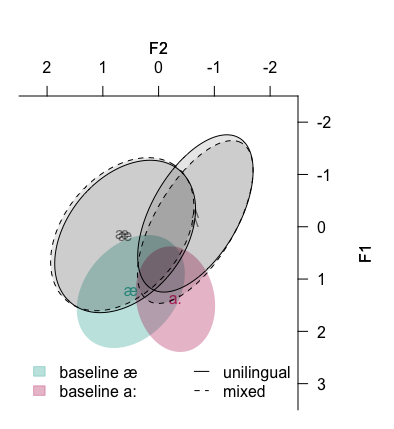
\includegraphics[scale=1]{vowels_e_b_final}
	\caption{Vowel quality in unilinual English, mixed, and baseline Bengali productions}
	\label{vowels_e_b}
\end{figure}

\newpage

\begin{figure}[h] %\centering
	
	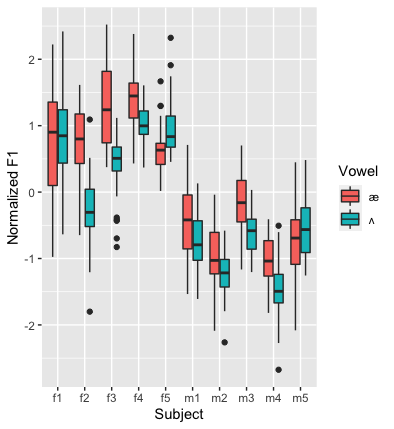
\includegraphics[scale=1]{vowel_by_subject_ggplot}
	\caption{Subject-wise mean F1 in unilingual English productions}
	\label{boxplot_F1}
\end{figure}

\end{document}
%%% Local Variables:
%%% mode: latex
%%% TeX-master: t
%%% TeX-engine: luatex
%%% End:
